
%(BEGIN_QUESTION)
% Copyright 2012, Tony R. Kuphaldt, released under the Creative Commons Attribution License (v 1.0)
% This means you may do almost anything with this work of mine, so long as you give me proper credit

A Programmable Logic Controller (PLC) serves as the logic solver (safety shutdown controller) for a large motor-driven pump.  It is programmed to shut off the pump if any dangerous conditions occur:

$$\includegraphics[width=15.5cm]{i02543x01.eps}$$

Red LED indicator lights on the input and output cards of the PLC indicate if those respective I/O channels are energized.  The light statuses shown in the above diagram are when the pump is running as it should (i.e. no abnormal conditions).

\vskip 10pt

Suppose this pump is running just as it should.  Identify how you could electrically simulate each of the following ``trip'' conditions, causing the pump to shut down even though nothing is physically wrong:

\begin{itemize}
\item{} Electrically simulate a condition of dangerous vibration to the PLC
\vskip 10pt
\item{} Electrically simulate an overloaded motor condition to the PLC
\vskip 10pt
\item{} Electrically simulate a condition of dangerous temperature to the PLC
\vskip 10pt
\item{} Electrically simulate a tripped PLC (to the motor contactor)
\end{itemize}


\vfil 

\underbar{file i02543}
\eject
%(END_QUESTION)





%(BEGIN_ANSWER)

This is a graded question -- no answers or hints given!

%(END_ANSWER)





%(BEGIN_NOTES)

Since we are told this pump is running as it should, with no abnormal conditions, we may assume that the discrete input conditions are exactly as they ought to be with no abnormal conditions detected.

\vskip 10pt

The vibration switch's input (X2) is unlit, which means that switch is presently open.  If this represents the ``good'' operating condition, then we may conclude a closed vibration switch represents a dangerous (shutdown) condition.  Thus, in order to simulate a condition of high vibration, we must short past the vibration switch with a jumper wire.

\vskip 10pt

The overload switch's input (X3) is lit, which means that switch is presently closed.  If this represents the ``good'' operating condition, then we may conclude an open overload switch represents a dangerous (shutdown) condition.  Thus, in order to simulate a condition of overload, we must open the overload switch circuit somewhere.

\vskip 10pt

The temperature switch's input (X4) is unlit, which means that switch is presently open.  If this represents the ``good'' operating condition, then we may conclude a closed temperature switch represents a dangerous (shutdown) condition.  Thus, in order to simulate a condition of abnormal temperature, we must short past the temperature switch with a jumper wire.  Incidentally, an abnormal temperature as defined by the configuration of this system is a {\it low} temperature, since the temperature switch is normally-closed and therefore will pass power to the PLC input only when the temperature falls below the trip setting.  Although it might be difficult to imagine a {\it cold} condition being dangerous to a pump, consider a case where the pump in question is located in an extremely cold environment (e.g. the North Slope oilfields in Alaska) and the temperature being monitored is the temperature of the lubricating oil.  Oil that is too cold will refuse to flow properly, which could damage the pump bearings more readily than oil that is too hot!


%INDEX% Safety, shutdown system: trip testing

%(END_NOTES)


